\documentclass{article}

\usepackage[final]{graphicx}
\usepackage{caption}
\usepackage{subcaption}
\usepackage[utf8]{inputenc}
\usepackage{amsmath}
\usepackage{amssymb}
\usepackage{anysize}
\usepackage{color}
\usepackage{xcolor}
\usepackage[]{algorithm2e}
\usepackage[framed,numbered,autolinebreaks,useliterate]{mcode}
\usepackage{floatrow}
\usepackage{listings}
\usepackage{algpseudocode}





\lstset{
	language=Matlab,                	% choose the language of the code
	basicstyle=\footnotesize,       % the size of the fonts that are used for the code
	numbers= left,                 	% where to put the line-numbers
	numberstyle=\footnotesize,      % the size of the fonts that are used for the line-numbers
	stepnumber=2,                   % the step between two line-numbers. If it is 1 each line will be numbered
	numbersep=5pt,                  % how far the line-numbers are from the code
	backgroundcolor=\color{white},  % choose the background color. You must add \usepackage{color}
	showspaces=false,               % show spaces adding particular underscores
	showstringspaces=false,         % underline spaces within strings
	showtabs=false,                 % show tabs within strings adding particular underscores
	frame=single,           		% adds a frame around the code
	tabsize=2,          			% sets default tabsize to 2 spaces
	captionpos=t,          			% sets the caption-position to bottom (t=top, b=bottom)
	breaklines=true,        		% sets automatic line breaking
	breakatwhitespace=false,    	% sets if automatic breaks should only happen at whitespace
	escapeinside={\%*}{*)}          % if you want to add a comment within your code
}



\usepackage{caption}
\DeclareCaptionFont{white}{\color{white}}
\DeclareCaptionFormat{listing}{\colorbox{gray}{\parbox[c]{\textwidth}{#1#2#3}}}
\captionsetup[lstlisting]{format=listing,labelfont=white,textfont=white}

\setlength\parindent{0pt}
\setlength{\parskip}{10pt}

\marginsize{3cm}{2cm}{2cm}{2cm}
%\documentclass[12pt]{article}

\begin{document}

\begin{titlepage}

\newcommand{\HRule}{\rule{\linewidth}{0.5mm}} % Defines a new command for the horizontal lines, change thickness here

\center % Center everything on the page
 
%----------------------------------------------------------------------------------------
%	HEADING SECTIONS
%----------------------------------------------------------------------------------------

\textsc{\LARGE Master Computer Vision}\\[1.5cm] % Name of your university/college
\textsc{\Large Scene Segmentation and Interpretation}\\[0.5cm] % Major heading such as course name


%----------------------------------------------------------------------------------------
%	TITLE SECTION
%----------------------------------------------------------------------------------------

\HRule \\[0.4cm]
{ \huge \bfseries Image Characterization}\\[0.4cm] % Title of your document
\HRule \\[1.5cm]
 
%----------------------------------------------------------------------------------------
%	AUTHOR SECTION
%----------------------------------------------------------------------------------------

\begin{minipage}{0.4\textwidth}
\begin{flushleft} \large
\emph{Author:}\\
Muhammad \textsc{Usman} % Your name
\\
Emre Ozan \textsc{Alkan}\\
Priyanka \textsc{Phutane}

\end{flushleft}
\end{minipage}
~
\begin{minipage}{0.4\textwidth}
\begin{flushright} \large
\emph{Course Co ordinator:} \\
Pere Ridao \textsc{Smith} % Supervisor's Name
\end{flushright}
\end{minipage}\\[4cm]

% If you don't want a supervisor, uncomment the two lines below and remove the section above
%\Large \emph{Author:}\\
%John \textsc{Smith}\\[3cm] % Your name

%----------------------------------------------------------------------------------------
%	DATE SECTION
%----------------------------------------------------------------------------------------

%{\large \today}\\[3cm] % Date, change the \today to a set date if you want to be precise

%----------------------------------------------------------------------------------------
%	LOGO SECTION
%----------------------------------------------------------------------------------------

%\includegraphics{Logo}\\[1cm] % Include a department/university logo - this will require the graphicx package
 
%----------------------------------------------------------------------------------------

\vfill % Fill the rest of the page with whitespace
\end{titlepage}

\section{Introduction and Problem Statement:}
In everyday life Texture means roughness, smoothness etc. which refers to feel. A texture which is considered as rough has a large difference between its highs and lows. This difference will be close to size of fingers so one feels it. Similarly for smooth texture this difference will be very small.It works similarly in Images the difference is now highs and lows are brightness values.So In imaging world texture means a certain pattern which occurs repetitively in images.[1] Texture analysis can be used for image segmentation and can be used in the variety of applications, including remote sensing, automated inspection, and medical image processing.[2] The goal of this lab is to study and implement the statistical methods to extract the image texture descriptors which can be used further for image segmentation.\\
In this lab we will use two methods for the extracting the image descriptors. In first method we will use the Grey Level Co-occurrence Matrix (GLCM)[2] and extracts values for Contrast, Homogeneity, Energy, and Entropy. As our goal will be to display these texture descriptors in the form of image so we will calculate them for every pixel and display the corresponding images. In the second part we are using the Energy Filter (Law mask) which gives us the static measures (mean, abs mean, and standard deviation) which are derived for each pixel and corresponding results are displayed.
\section{Algorithm Analysis:}
Now we will discuss the two algorithms we used for calculating texture descriptors. 
\subsection{Gray Level Co-occurrence Matrix }
The GLCM is a tabulation of how often different combinations of pixel brightness values (grey levels) appear in an image.[1] First order texture measures are calculated from the original image values e.g. variance and do not depend upon the relation of pixel with its neighbourhood. Second order texture measures depend upon the relationship between group of two pixels. The Algorithm described here will be used to calculate second order texture measures.[1]
\subsubsection{Spatial Relationship between two pixels:}
GLCM algorithm considers the relationship between two pixels at a time. One pixel is called reference and other is called neighbour. One can choose neighbourhood by mean of vector and then each pixel in window (which is specified and changes will be considered inside that window only) will become reference and by doing so entries of GLCM matrix will be filled.[1]
\subsubsection{Separation between two pixels:}
One can also specify the distance between reference and neighbourhood pixels to be considered while calculating GLCM commonly known as offset. Commonly we use 1 as offset which means immediate neighbour of reference pixel. Care should be taken while selecting offset as it should be less than window size.[1]
\subsubsection{Other Parameters:}
The Co-occurrence matrix also depend upon window size we will use to compute GLCM matrix for certain pixel. It also depend upon the number of grey levels we want to use to build matrix as there can be wide range of grey levels present in image and if we dont reduce the size of image then the size of co-occurrence matrix will be big so we want to scale down to make computation faster.[1]
\subsubsection{Computing GLCM Matrix:}
We construct our Co-occurrence matrix by simply considering our window specified by window size parameter. We take its centre pixel and move it to pixel for which we want to measure co-occurrence matrix. Now we will count pairs of pixels specified  by taking into account the specified offset and spatial relationship.[1]
\begin{table}[H]
    \begin{tabular}{|l|l|l|l|}
    \hline
    0 & 0 & 1 & 1 \\ \hline
    0 & 0 & 1 & 1 \\ \hline
    0 & 2 & 2 & 2 \\ \hline
    2 & 2 & 3 & 3 \\ \hline
    \end{tabular}
    \caption{Sample Image}
\end{table}
Now we will show the co-occurrence matrix using distance 1 and Angle 0. One thing should be noted that we have taken care of symmetry while building this matrix. It will be different if we don't consider symmetry.
\begin{table}[H]
    \begin{tabular}{|l|l|l|l|l|}
    \hline
    Neighbourhood Pixel \textrightarrow & 0 & 1 & 2 & 3 \\
    Reference Pixel \textdownarrow       & ~ & ~ & ~ & ~ \\ \hline
    0                     & 2 & 2 & 1 & 0 \\ \hline
    1                     & 0 & 2 & 0 & 0 \\ \hline
    2                     & 0 & 0 & 3 & 1 \\ \hline
    3                     & 0 & 0 & 0 & 1 \\ \hline
    \end{tabular}
    \caption{Co-occurrence Matrix using Distance 1 and Angle $0\deg$ [1]}
\end{table}
\subsubsection{Reading GLCM Matrix:}
The first(top left) element of the matrix will always be filled with number of times combination (0,0) occurs which means how many times within image area a pixel with grey level 0(neighbour pixel) appears to the right of another pixel with grey level 0(reference pixel).[1] Different co-occurrence matrix exist for each spatial relationship.\\
\\
Now we have computed our co-occurrence matrix for pixel on which our window was centred. Now we can use this matrix to measure different statistics given below.\\
\underline{Contrast:}\\
Contrast is the measurement of the difference between pixel value and its neighbour value computed for entire image.Higher values of contrast indicate large variation in image intensities while low value indicate image is quite homogenius having small changes in intensities. Formula for calculating contrast is given below.
\[ Contrast = \sum_{i,j=0}^{N-1}(i - j)^{2} \times m_{i j} \]
\underline{Homogeneity:}\\
Homogeneity is the quantitative measure of state of co-occurrence matrix being homogenius or uniform. The formula for calculation of homogeneity is given below.
\[ Homogeneity = \sum_{i,j=0}^{N-1}\frac{m_{ij}}{1+\left | i-j \right |} \]
\\
\underline{Entropy:}\\
Entropy is the measurement of randomness among the co-occurrence matrix elements. The formula for calculation of entropy is given below.
\[ Entropy = \sum_{i,j=0}^{N-1}m_{ij}\times \log \left ( m_{ij} \right ) \]
\\
\underline{Energy:}\\
The energy of co-occurrence matrix is calculated by the formula given below.
\[ Energy=\sum _{i,j=0}^{N-1}m_{ij}^{2} \]
\subsection{Energy Filters:}
We can measure the texture energy by using Laws' method of texture
energy transforms. To do so first of all we convolve our image with 2d Law's Mask. The output form these texture energy filters. These consist of moving window calculation of variance or more cheaply a moving window average of absolute values.[3] The 2d kernels used for convolution are primarily derived from one dimensional filers given below.
\begin{table}[H]
    \begin{tabular}{|l|l|}
    \hline
    1 x 3 Filters  & 1 x 5 Filetrs       \\ \hline
    L3 = [1 2 1]   & L5 = [1 4 6 4 1]    \\ \hline
    E3 = [-1 0 1]  & E5 = [-1 -2 0 2 1]  \\ \hline
    S3 = [-1 2 -1] & S5 = [-1 0 2 0 -1]  \\ \hline
    ~              & R5 = [1 -4 5 -4 1]  \\ \hline
    ~              & W5 = [-1 2 0 -2 -1] \\ \hline
    \end{tabular}
    \caption{Primitive 1 Dimensional Filters}
\end{table}
\section{Design and Implementation:}
We implemented both algorithms in Matlab. Now we will discuss the implementation issues of both algorithm individually.
\subsection{GLCM Algorithm:}
As we stated before we used Matlab to implement our algorithm so we take benefit of built in Matlab function to implement our GLCM Algorithm. We  used two important Matlab functions named "graycomatrix", which returns co-occurrence matrix for image according the parameters passed to it and "graycoprops" function which provide us required statistical measures for the passed co-occurrence matrix. Now we will explain the different parameters of these functions.
\subsubsection{Parameters of "graycomatrix"}
Below is the explanation of different input parameters of "graycomatrix".
\\
\underline{\textbf{Offset:}}\\
 It is used to specify the distance and the orientation from pixel of interest(reference pixel) and the neighbour. The following table shows the orientation  and corresponding offset for a given distance.
 \begin{table}[H]
     \begin{tabular}{|l|l|}
     \hline
     \textbf{Angle} & \textbf{Offset}  \\ \hline
     0     & [0 D]   \\ \hline
     45    & [-D D]  \\ \hline
     90    & [-D 0]  \\ \hline
     135   & [-D -D] \\ \hline
     \end{tabular}
     \caption{Offset and Orientation Chart}
 \end{table}
  \underline{\textbf{Numlevel:}}\\
 This parameter allows us to set the number of grey levels to be used while scaling the grey level values to sub image.It can take values between 1 and 8.[2]
 \\
  \underline{\textbf{Symmetry:}}\\
  This parameter take two values true or false. If it is set then Matlab take into account the ordering of values in pixel pairs.[2]
  \subsubsection{Parameters of " graycoprops"}
  This function take GLCM matrix as input and name of desired property we want to find. The properties are Contrast, Energy, Correlation and Homogeneity.\\
  Entropy of the Image can be calculated using Matlab function "\textbf{entropyfilt}" and is independent from graycoprops" function.\\
  The Pseudo Code for our Implementation of GLCM is given below.

\begin{algorithm}[H]
 \KwData{Gray scale ‘image’.}
 \KwResult{Entropy, Contrast, Correlation, Energy and Homogeneity images of the input 'image' .}
 Calculate 'entropyImage' with ‘entropyfilt’ function;
 Initialize ‘windowSize’ with odd number preferably 7 or 9\;
 Initialize ‘windowCenter’ with floor of half of ‘windowSize’\;
 Pad the ‘image’ borders with size of ‘windowCenter’\;
 Initialize ‘offset’ with vector in form of  [0 D], [-D, D], [-D, 0,], [-D, -D]\; 
 Initialize ‘numLevels’ with 8\;
 Initialize ‘symmetric’ with false or true\;
 Initialize ‘contrastImage’ as size of ‘image’ with zeros\; 
 Initialize ‘correlationImage’ as size of ‘image’ with zeros\; 
 Initialize ‘energyImage’ as size of ‘image’ with zeros\; 
 Initialize ‘homogeneityImage’ as size of ‘image’ with zeros\; 
 
 Initialize ‘rows’ and ‘cols’ with ‘image’ size\;
 
 \For{$i\leftarrow (‘windowCenter’ + 1)$ \KwTo $(‘rows’ - ‘windowCenter’)$}
 {
 	 \For{$j\leftarrow (‘windowCenter’ + 1)$ \KwTo $(‘cols’ - ‘windowCenter’)$}
 	 {
 	 	Get ‘subImage’ as size of ‘windowCenter’ from ‘image’ with center $i$ and $j$\;
 	 	Compute ‘GLCM’ with ‘graycomatrix’ function as input ‘subImage’\;
 	 	Compute ‘contrast’, ‘correlation’, ‘energy’ and ‘homogeneity’ with ‘graycoprops’ function as input ‘GLCM’
 	 	Set ‘contrastImage’ pixel($i$, $j$) with ‘contrast’\;
 	 	Set ‘correlationImage’ pixel($i$, $j$) with ‘correlation’;
 	 	Set ‘energyImage’ pixel($i$, $j$) with ‘energy’;
 	 	Set ‘homogeneityImage’ pixel($i$, $j$) with ‘homogeneity’;
 	 }
 }
 
 Remove paddings of ‘image’, ‘contrastImage’, ‘correlationImage’, ‘energyImage’ and ‘homogeneityImage’\;
 
 \caption{GLCM Algorithm}
\end{algorithm}  
  
\subsection{Energy Filters:}
The pseudo Algorithm is given below.

\begin{algorithm}[H]
 \KwData{Colored  ‘image’.}
 \KwResult{Laws' filter ans statistics  of the input ‘image’ .}
Separate RGB channels of the ‘image’ as  ‘imageR’,  ‘imageG’,  ‘imageB’\;
Initialize ‘imageGray’ with gray level of the  input ‘image’\;
Initialize  ‘hsvImage’ with color conversion from RGB of ‘image’\;
Initialize  ‘hueImage’ from ‘hsvImage’'s first channel\;
Initialize lawsMask with some mask\;

Convolve ‘imageGray’, ‘imageR’, ‘imageG’, ‘imageB’,  and ‘hueImage’ with Laws' mask\;
Show the results\;

Initialize ‘filterSize’ with odd number preferable 7 or 9\;

Find mean of the ‘imageGray’, ‘imageR’, ‘imageG’, ‘imageB’,  and ‘hueImage’\;

Initialize ‘meanOutputImage’ with combination of mean of ‘imageGray’, ‘imageR’, ‘imageG’\;

Show the mean results\;

Find absolute mean of the ‘imageGray’, ‘imageR’, ‘imageG’, ‘imageB’,  and ‘hueImage’\;

Initialize ‘absmeanOutputImage’ with combination of absolute mean of ‘imageGray’, ‘imageR’, ‘imageG’\;

Show the absolute mean results\;

Find standart deviation of the ‘imageGray’, ‘imageR’, ‘imageG’, ‘imageB’,  and ‘hueImage’\;

Initialize ‘stdDevOutputImage’ with combination of standart deviation of ‘imageGray’, ‘imageR’, ‘imageG’\;

Show the standart deviation esults\;

 \caption{Energy Filters Algorithm}
\end{algorithm}

%\begin{itemize}
%  \item[1] We may randomly select seed and grow it until no more pixels fulfil the aggregation criteria and then select another seed randomly from unassigned pixels and keep repeating this process until all the pixels get assigned to some region. This method is useful when image under consideration is of complex nature.
%  \item[2] We may manually input the certain number of seeds to algorithm. This can be useful when the image is simple and we want to segment desired regions.
%  \item[3] We may utilize image information to select and place seeds appropriately. The strategy we devise is to select the local peaks from the histogram and find corresponding intensity value and then select any pixel of that intensity as seed point. We do this for all local peaks and then if some parts of image left un assigned randomly select seed from them. But this method is useful only in case of simple images.
%
%\end{itemize}
%\subsection{Type of Adjacency for Neighbourhood:}
%We can choose either eight or four Adjacency for selecting neighbourhood but one thing should be kept while selecting that using eight Adjacency will take more time to process.
%\subsection{Aggregation Criteria:}
%This is the most important and difficult question to answer. There can be number of ways to select the aggregation criteria. Below we enlisted the criteria we used in our implementations.
%\begin{itemize}
%  \item[1] The first method can be simply take mean of current region and check if intensity of test pixel is inside range, mean plus minus certain threshold or not. If its inside we add it to our region. This threshold is very important as it decides the sensitivity of aggregation criteria.
%  \[ \mu_{c} - X < I_{x} < \mu_{c} + X \]
%  Where $ I_{x} $ is our test pixel, X is Threshold to selected empirically and $\mu_{c}$ is mean of current region.
%  \item[2] We can also calculate mean and standard deviation of the current region. Now we will add test pixel which is being tested for aggregation criteria if it fulfils given condition.
%   \[ \mu_{c} - X\sigma_{c} < I_{x} < \mu_{c} + X\sigma_{c} \]
%     Where $ I_{x} $ is our test pixel, X is Threshold to be selected empirically,$\sigma_{c}$,$\mu_{c}$ is standard deviation and mean of current region.
%  \item[3] For an RGB image we can find mean and standard deviation of three channels separately and then take mean of all standard deviations and use that value as shown below.
%   \[ \mu_{c} - X\sigma_{c} < I_{x} < \mu_{c} + X\sigma_{c} \]
%   Where,
%   \[\mu_{c} = \frac{\mu_{cr} + \mu_{cg} + \mu_{cb}}{3} \]
%   and,
%   \[\sigma_{c} = \frac{\sigma_{cr} + \sigma_{cg} + \sigma_{cb}}{3} \]
%   $\sigma_{c}$ is average of standard deviation of all channels and $\mu_{c}$ is average of means of all channels.
%\end{itemize}



%\section{Design and Implementation:}
%There is two main part for this lab. One with using co-occurence matrices, and other with energy filtes. For co-occurence matrices, we tried to design our program 
%
%
%%We used Matlab for implementing and testing our segmentation algorithm. We used queue to explore neighbours. When we explore neighbours of pixel we add them to queue and then we check them against aggregation criteria if they agree we add them to region and remove from queue and repeat this process until our queue goes empty or region reaches its maximum area under the given aggregation criteria.\\
%%For labelling the regions we create another matrix called region matrix of the same size as original image and when some pixels fulfils the aggregation criteria we label it in region matrix. And this matrix will be used at end as a result of segmentation. Also we will maintained a visited matrix which is also of same size as original image. When ever some pixel is assigned to certain region we will make corresponding pixel in visited matrix 1. We will use eight adjacency in our implementations.\\
%%\\
%%Add Pseudo Code here\\
%%\\
%%When our algorithm is finished with segmentation we change labels to random colours so that we can visualize our results of segmentation in a better way. TO compare our results with ground truth we convert our segmented result to binary image and find specificity and sensitivity.




\subsection{Functions Developed:}

	\begin{itemize}
		\item FindImageMean Function: Gets image and filter size, and convolve image with mean filter and normalize it.
		\item FindImageStdDev Function: Applies standard deviation filter on image with ‘stdfilt’ function of matlab. Then it normalizes the image.
		\item ImageMaskFilter: Convolve image with given filter and normalizes the image.
		\item CoOccurenceMatricesScript Script: Calculating entropy image, and contrast, correlation, energy and homogeneity of the each pixel. Then it shows the results.It uses ‘graycomatrix’, ‘graycoprops’ functions of matlab.
		\item EnergyFiltersScript Script: This script separated into 2 part. First, convolving image channels, gray image and hue image with Laws’ masks/filters and showing results. Later, it defines filter size and finding mean, absolute mean and standard deviation of the image channels, gray image and hue image. And then shows the result.
		
	\end{itemize}
		
		
	\begin{itemize}
		\item peakdet Function: Helper function to find peaks in vector from external author. We attempted to use this function to find peaks in histogram to select our seeds.
		\item FindSeed Function: At first, we tried to implement finding seeds in histogram peaks. So this function, getting grayscale image, region matrix and the peak values of the histograms. According to peaks, it find seeds in image, and checking if it is already in region or not. If not in any region, seed row and column index is returned. However due to limitation and complex images, we changed this function to just return first zero element in region matrix.
		\item TestScript Script: Test script for testing ‘RegionGrowingSegmentation’ function. It loads image, define neighborhood type and call the function.
		\item AddNeighbors Function: Adding 4 or 8 neighbors of given pixel index to passed neighbor list.  Image’s row and col count is sent for checking against out of boundary errors. Also visited matrix is provided to check if neighbor is visited before or not.
		\item ColorSegments Function: After image segmentation, region matrix has different labels/regions. We create same size colored image and for each unique region, we assign random color. Function getting region matrix as input and returning color segmented image and binary image. Binary image is created by finding most biggest region and making it black, which is mostly becomes background and rest is assigned to white.
		\item SegmentationEvaluation Function: Segmentation evaluation function is to calculate sensitivity and specificity which are statistical measures of the performance of a binary classification test. It gets segmented image, ground truth, and colors of the object and background and returns sensitivity and specificity.
		\item FindSeedFromUnlabeled Function: When histogram peaks are used to determine seeds, after FindSeed has no more returning seeds, we use this function to get seed. It gets region matrix as input and finding first zero value in region matrix and returning its indexes as output.
		\item CheckFixUnlabaledRegions.m Function: We stopped using this function since its time consuming. It gets region matrix as input, and returns it after finding some unlabeled pixels with zero value, and trying them to merge with near regions.
		\item RegionGrowingSegmentation Function: This is the main function, doing all the job. It gets image, optionally neighborhood type and returns color segmented image, binary image and labeled region matrix. When it finishes, before sending segmented image and binary image, we apply median filter, closing and opening morphological operations for better results.
		
	\end{itemize}


\section{Experimental Results and Analysis}

\subsection{GLCM Results}
%windowSize = 9; % 3 5 7 9 11 13 15 17 19 21
%offset = [-1 1];
%numLevels = 8;
%symmetric = false;

In this section we've taken results for one build-in Matlab image with different orientations like 0, 45, 90, 135. Other parameters like windows size, numlevels, symmetric are let to default 9, 8 and false respectively.

Here are the results 6 images; original, entropy, contrast, correlation, energy and homogeneity.

\begin{figure}[H]
\begin{center}
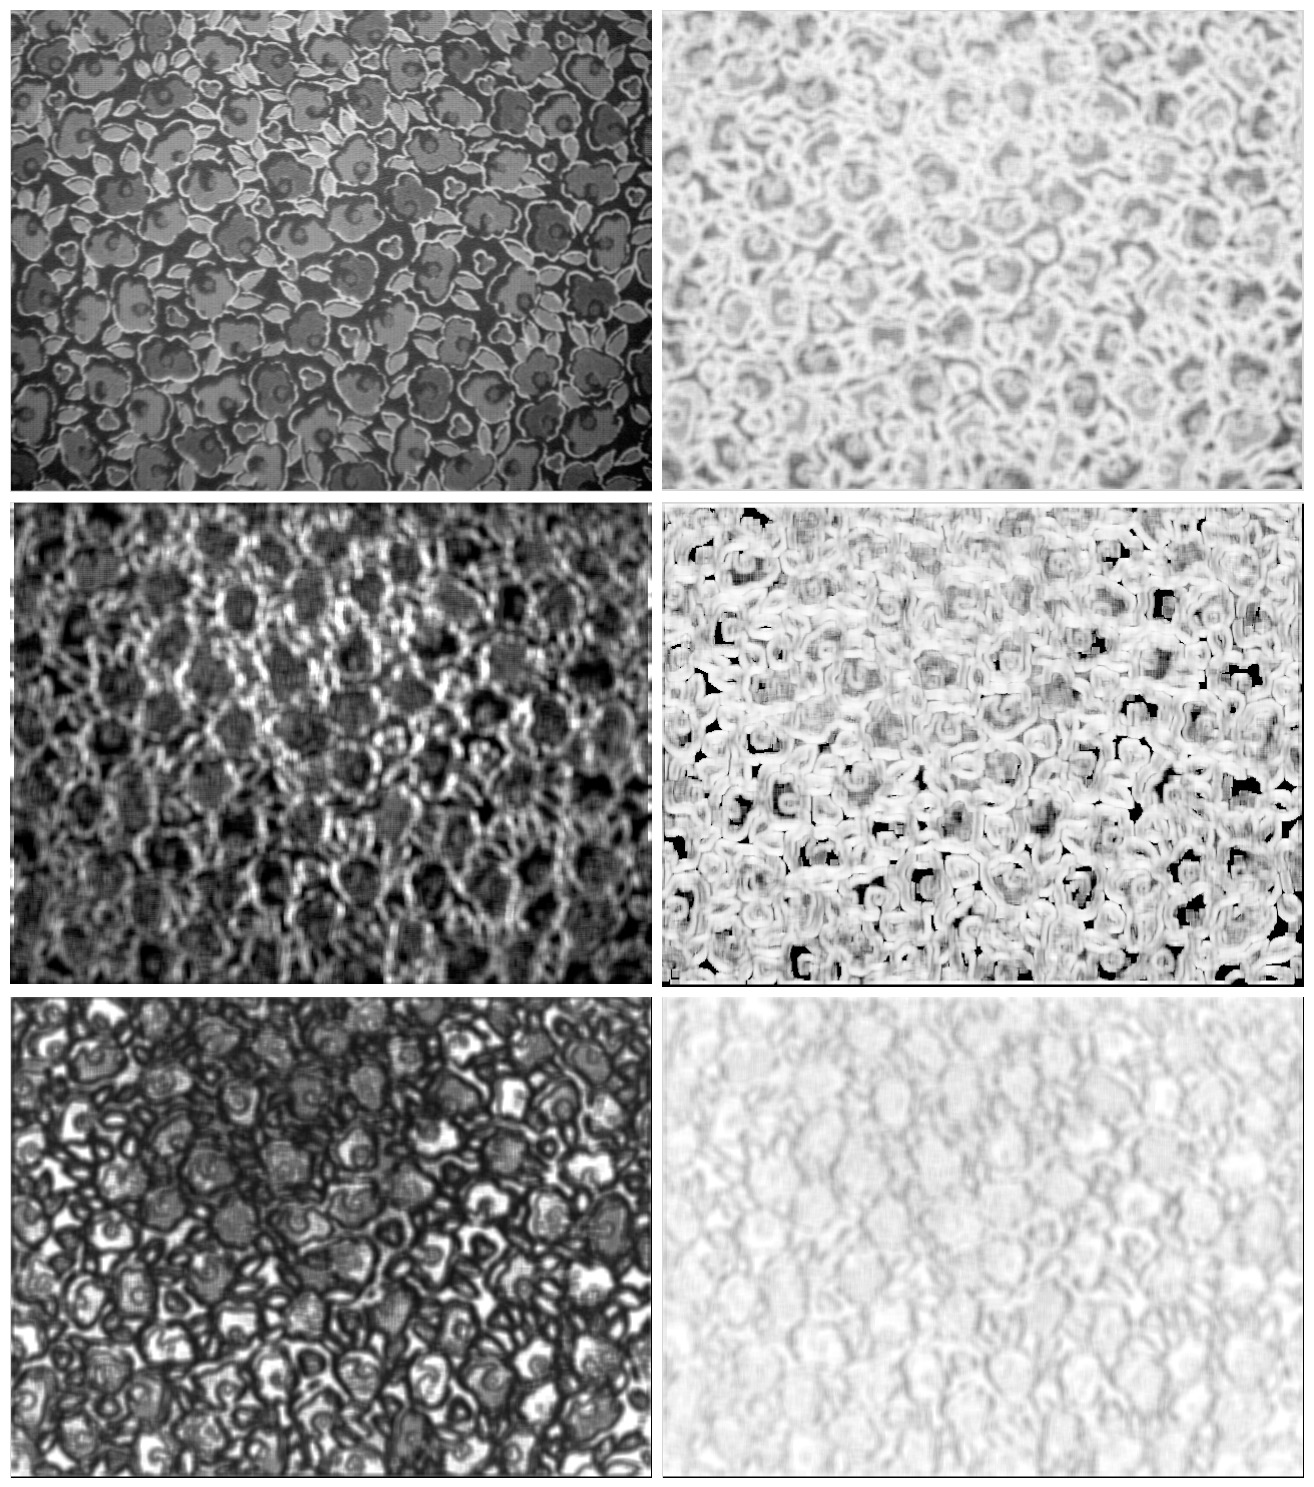
\includegraphics[scale=0.35]{result1.jpeg}
\caption{Results with 0 degree}
\end{center}
\end{figure}	

\begin{figure}[H]
\begin{center}
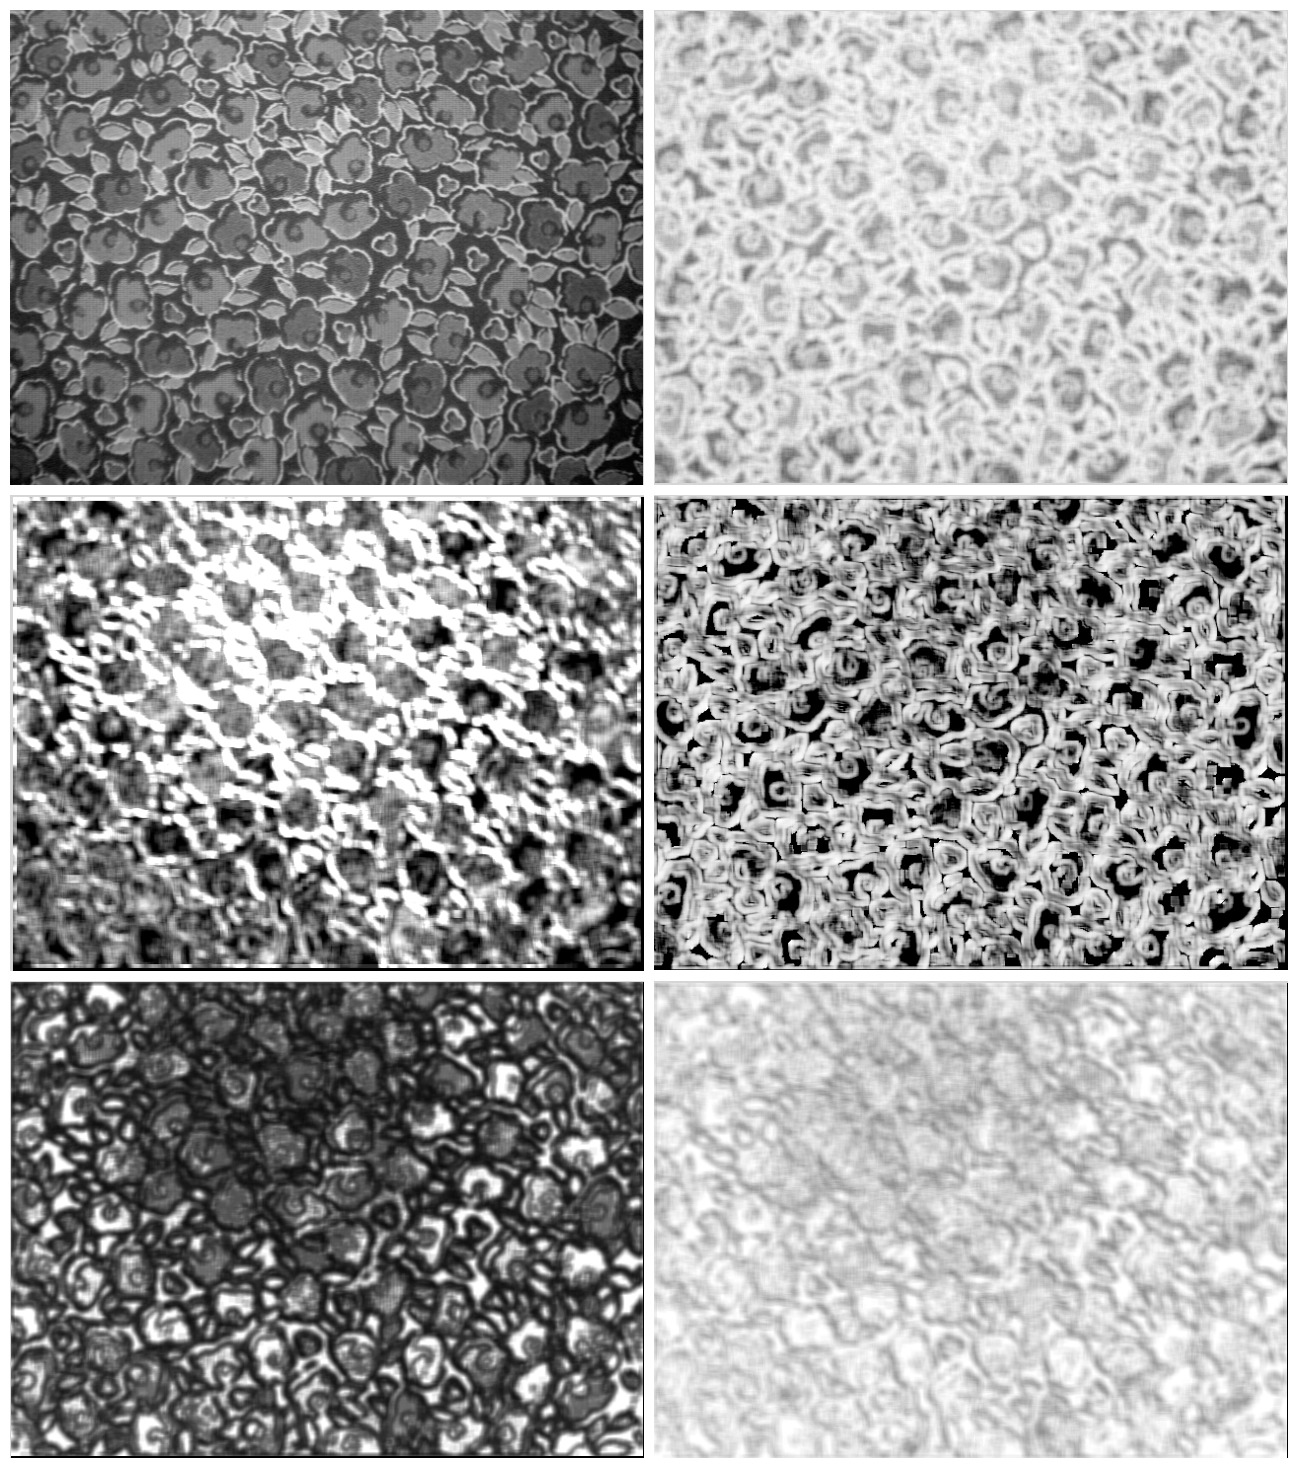
\includegraphics[scale=0.35]{result2.jpeg}
\caption{Results with 45 degree}
\end{center}
\end{figure}	

\begin{figure}[H]
\begin{center}
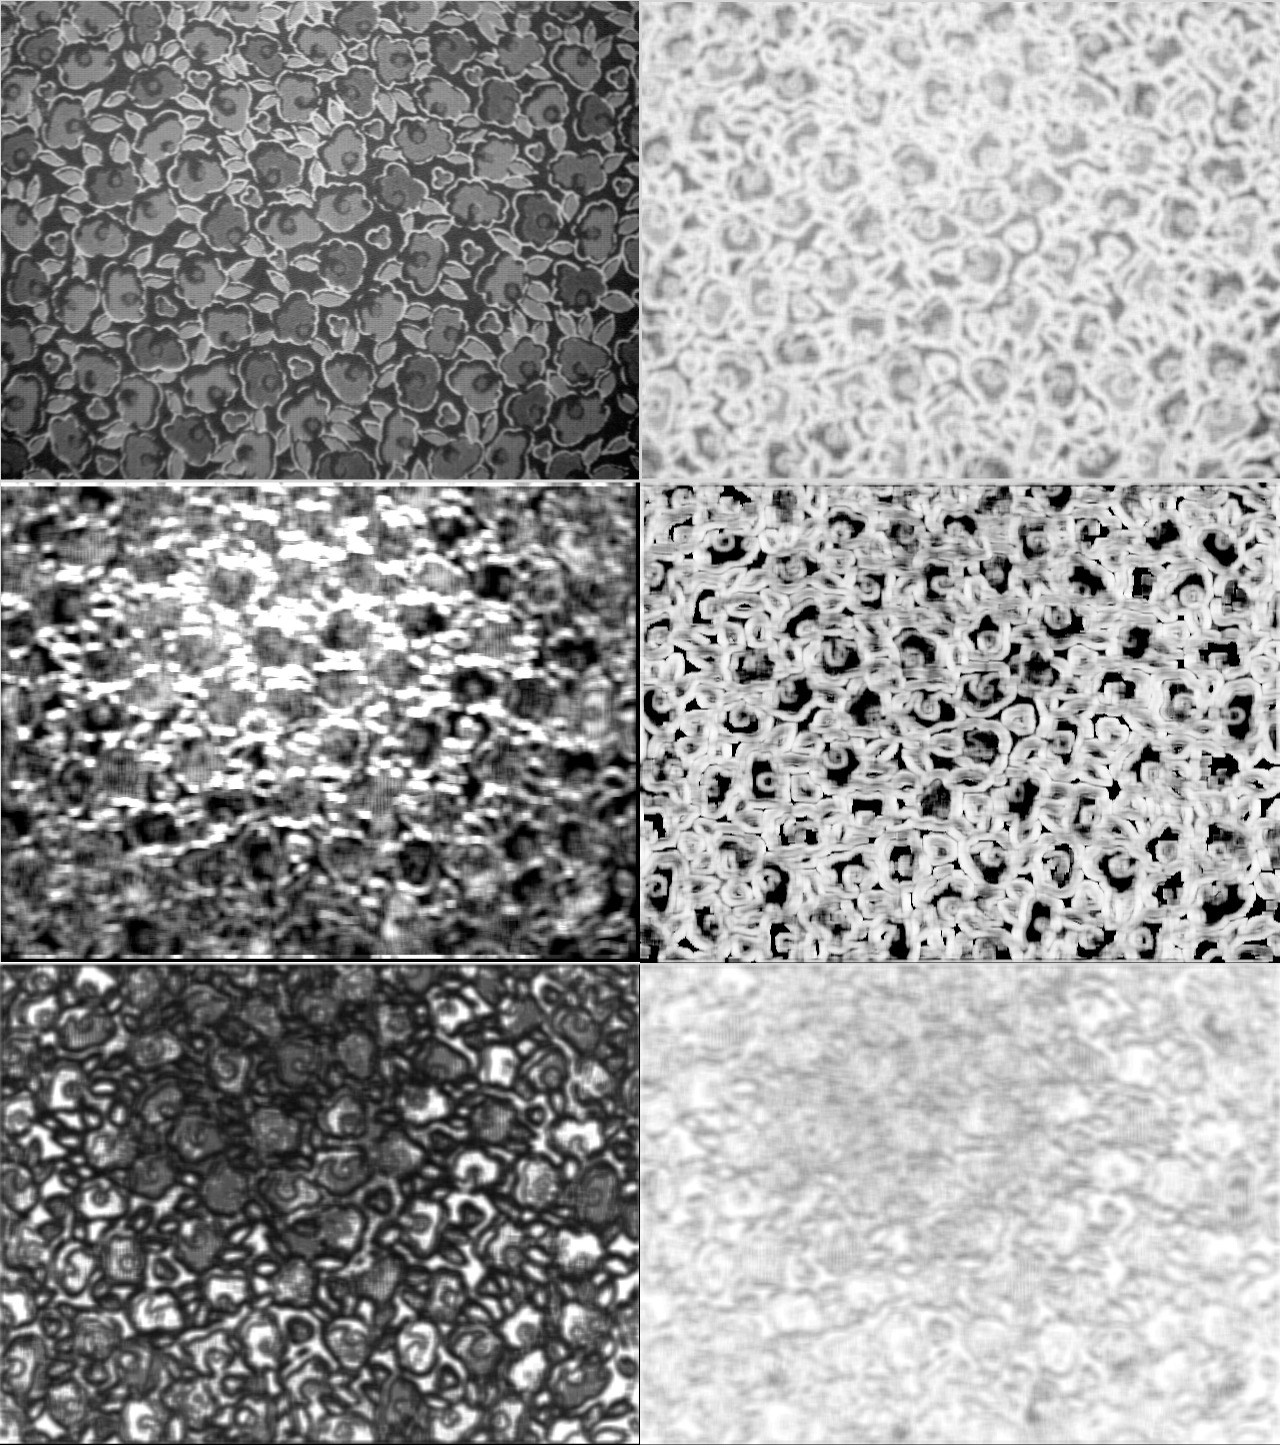
\includegraphics[scale=0.35]{result3.jpeg}
\caption{Results with 90 degree}
\end{center}
\end{figure}	

\begin{figure}[H]
\begin{center}
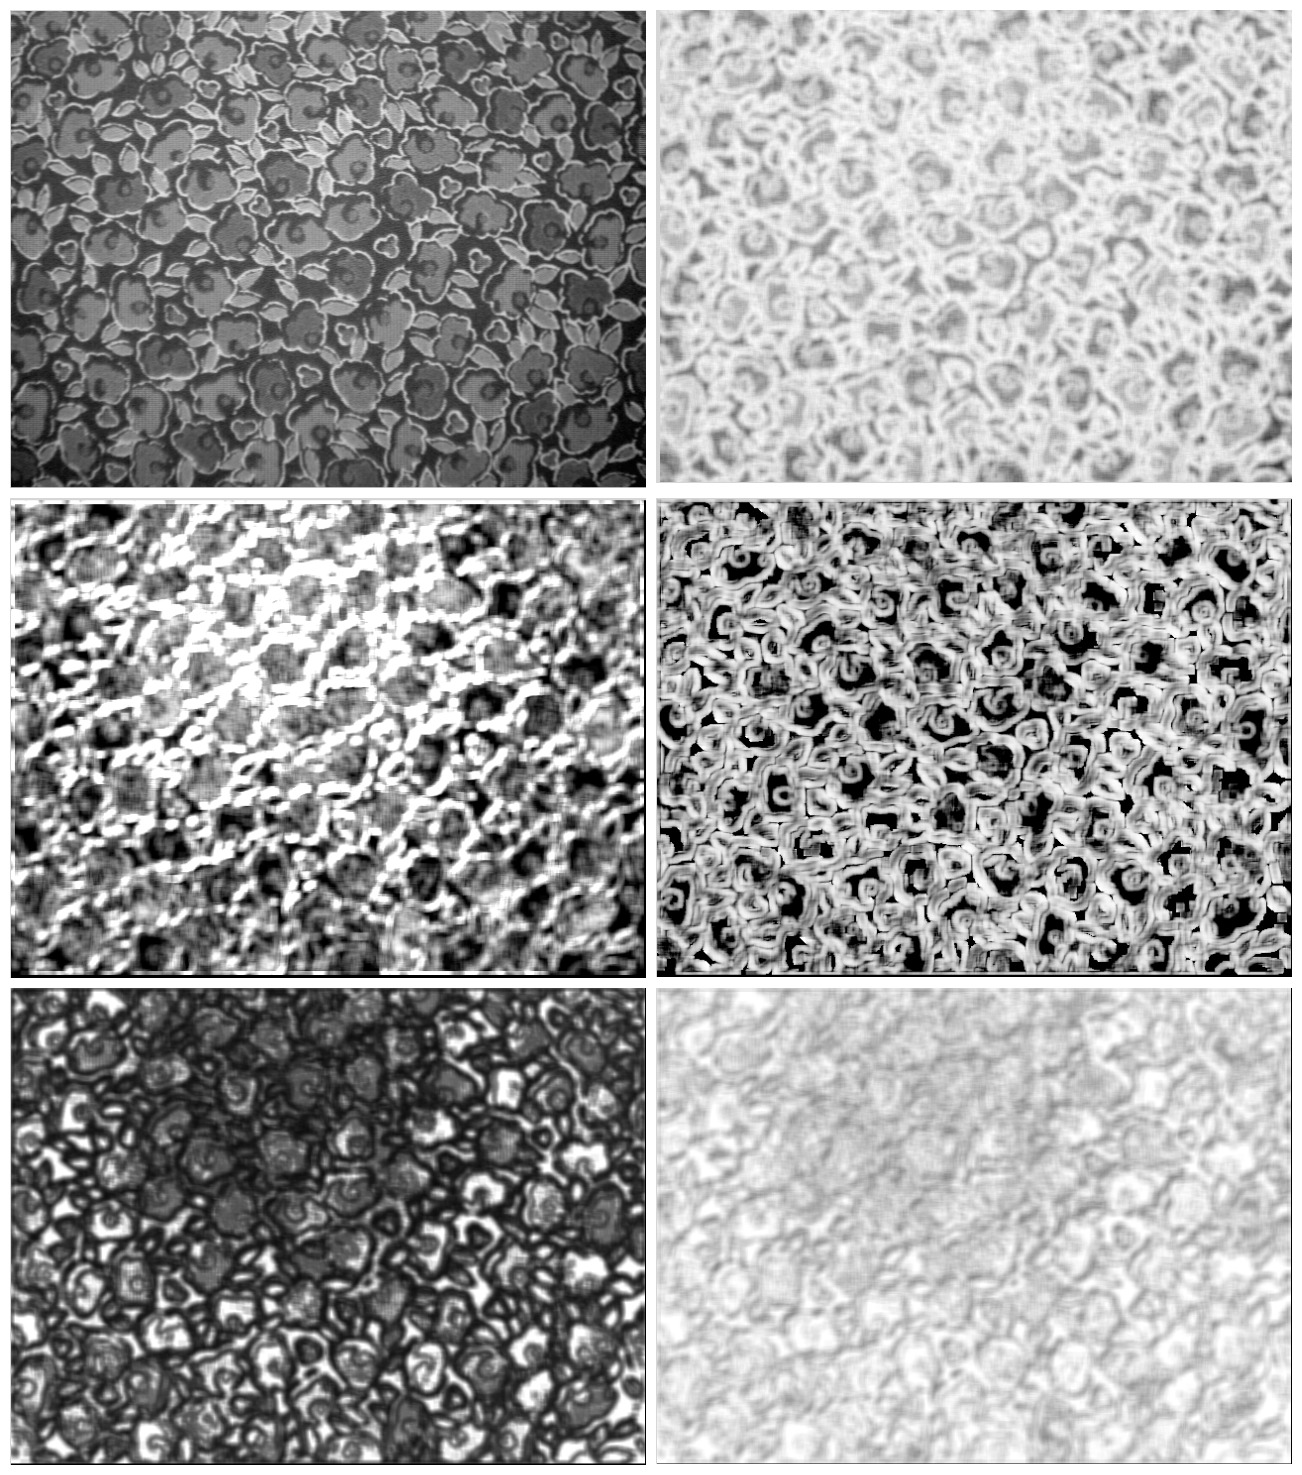
\includegraphics[scale=0.35]{result4.jpeg}
\caption{Results with 135 degree}
\end{center}
\end{figure}	

\subsection{Mean, Absolute Mean and Std.Dev. Results}
In this section we calculated results with applying mean, absolute mean, standart deviation and normalization of the images of its channels, gray level and hue.

Here is the results:

\begin{figure}[H]
\begin{center}
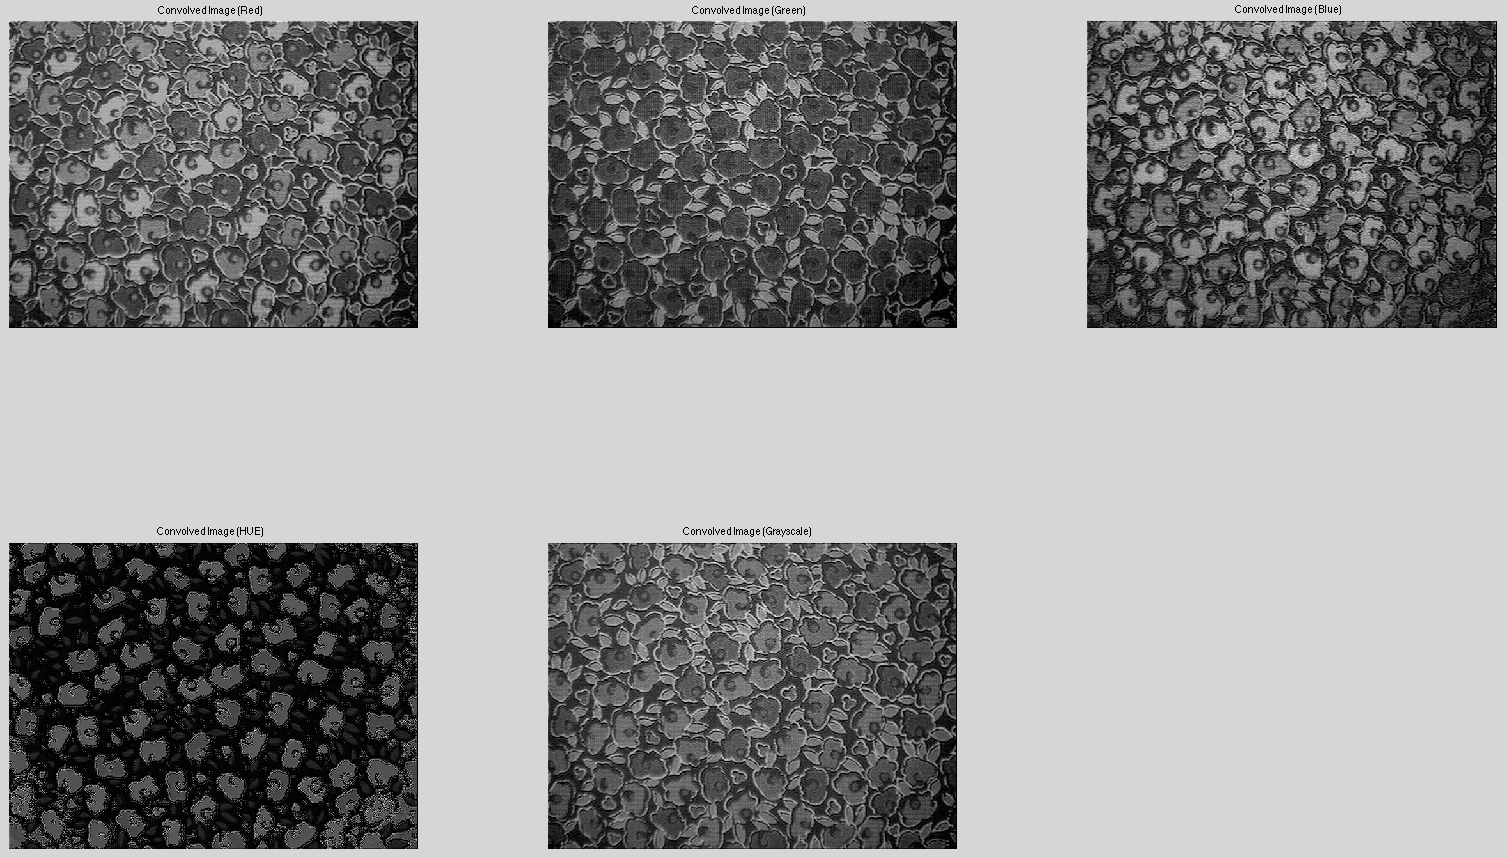
\includegraphics[scale=0.3]{lawsFilter.png}
\caption{Laws Filter convolution of R, G, B channels, HUE and grayscale}
\end{center}
\end{figure}	

\begin{figure}[H]
\begin{center}
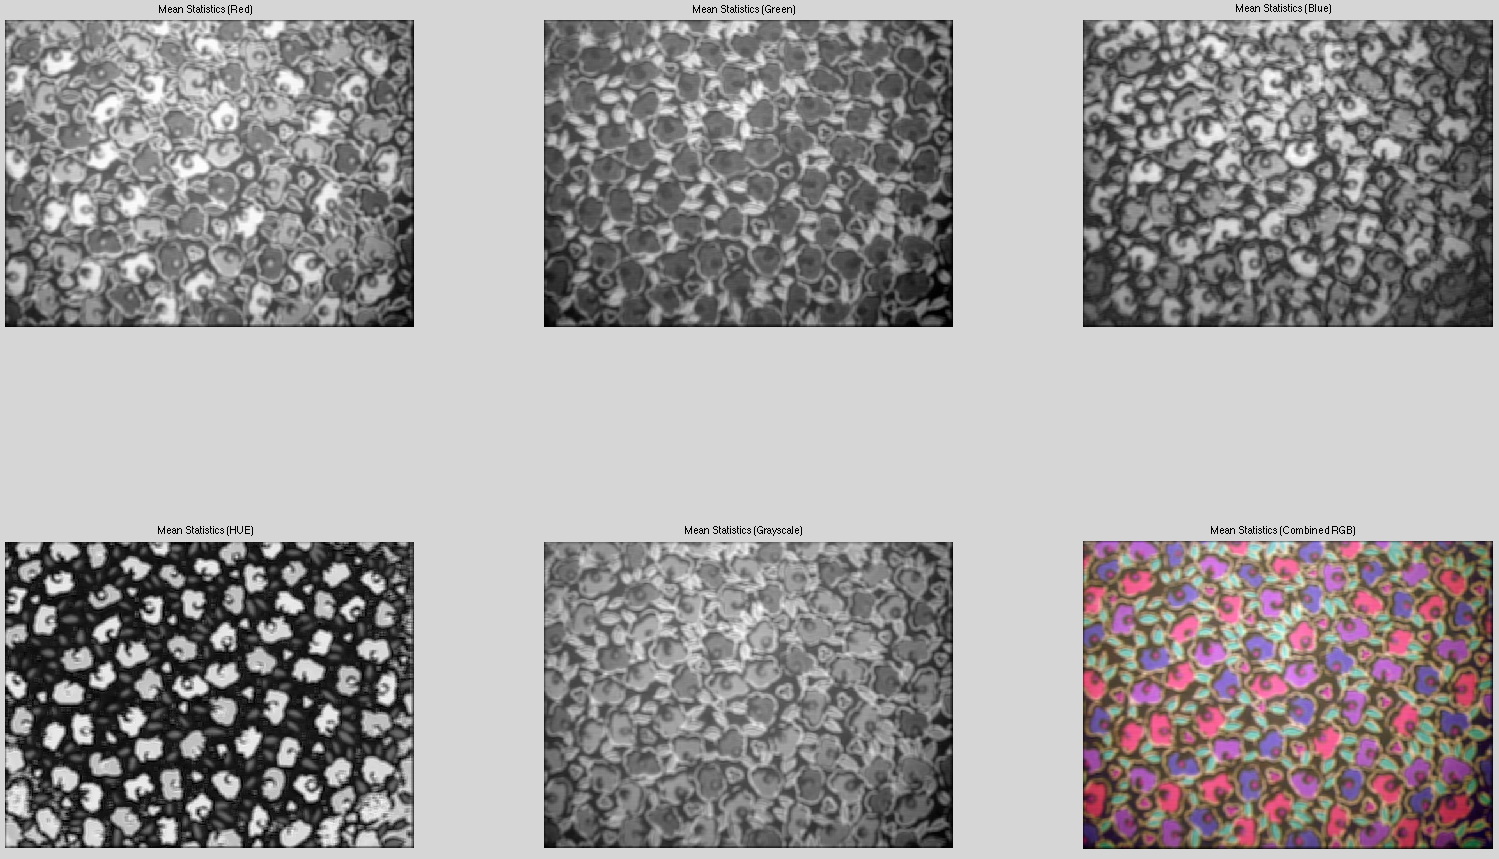
\includegraphics[scale=0.3]{meanStatistics.png}
\caption{Mean of R, G, B channels, HUE and grayscale}
\end{center}
\end{figure}	

\begin{figure}[H]
\begin{center}
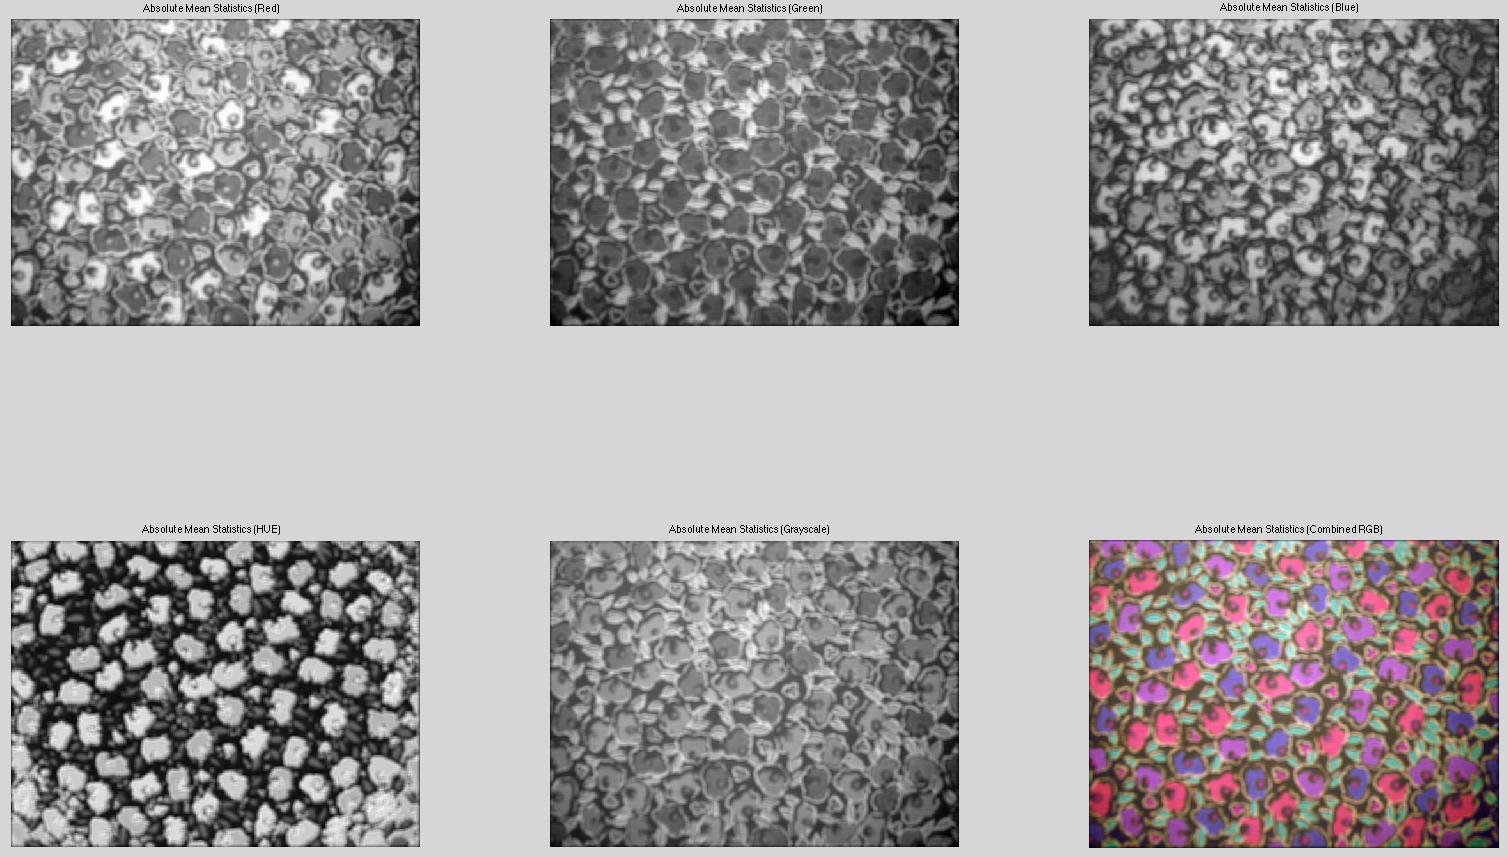
\includegraphics[scale=0.3]{absoluteMeanStatistics.png}
\caption{Absolute mean of R, G, B channels, HUE and grayscale}
\end{center}
\end{figure}	

\begin{figure}[H]
\begin{center}
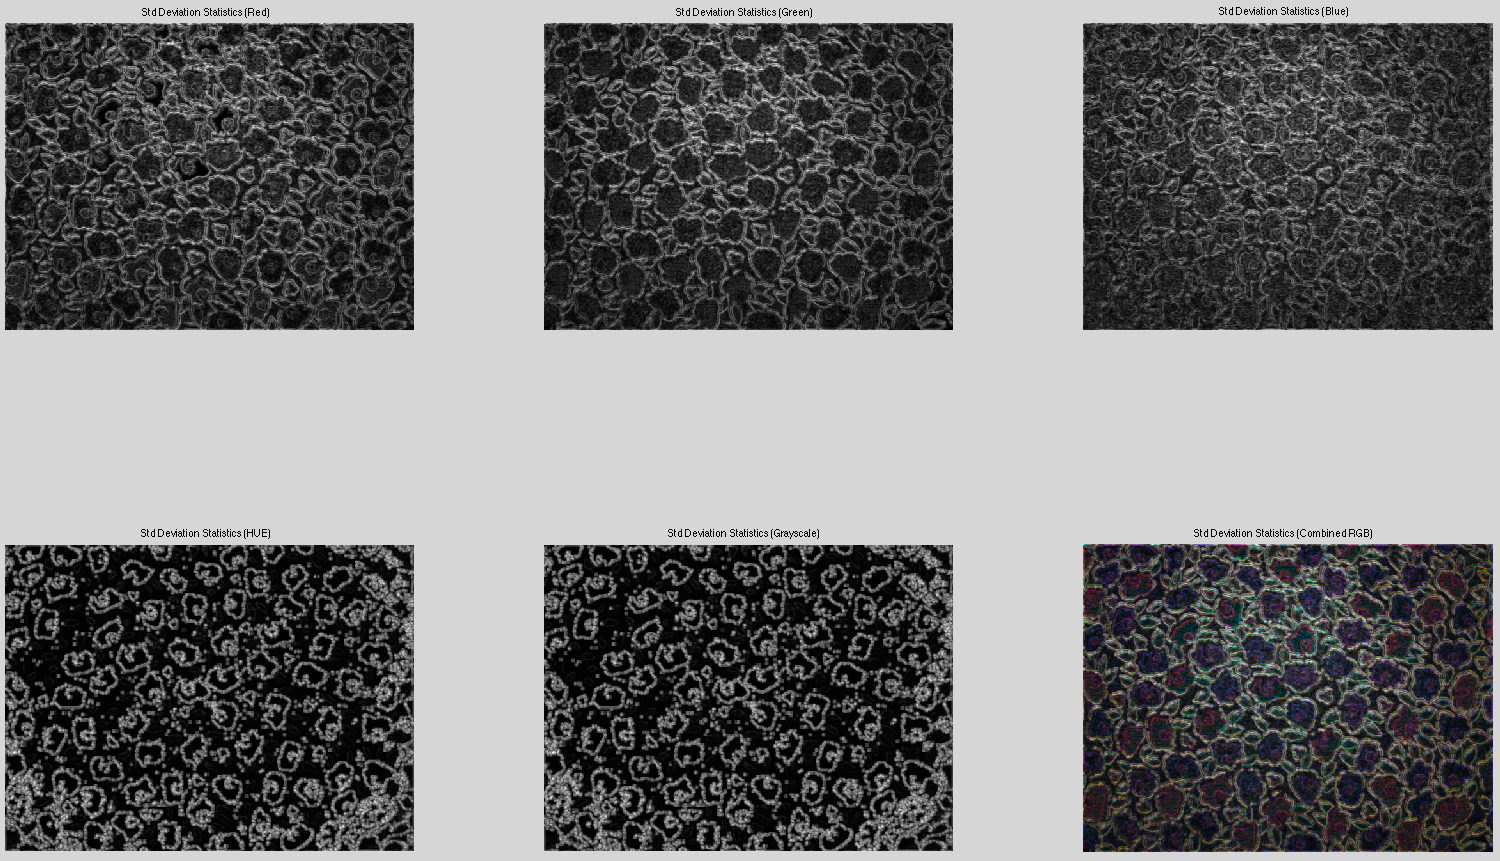
\includegraphics[scale=0.3]{standartDeviation.png}
\caption{Standart deviation of R, G, B channels, HUE and grayscale}
\end{center}
\end{figure}	




\subsection{Solution:}

%\begin{figure}[H]  
%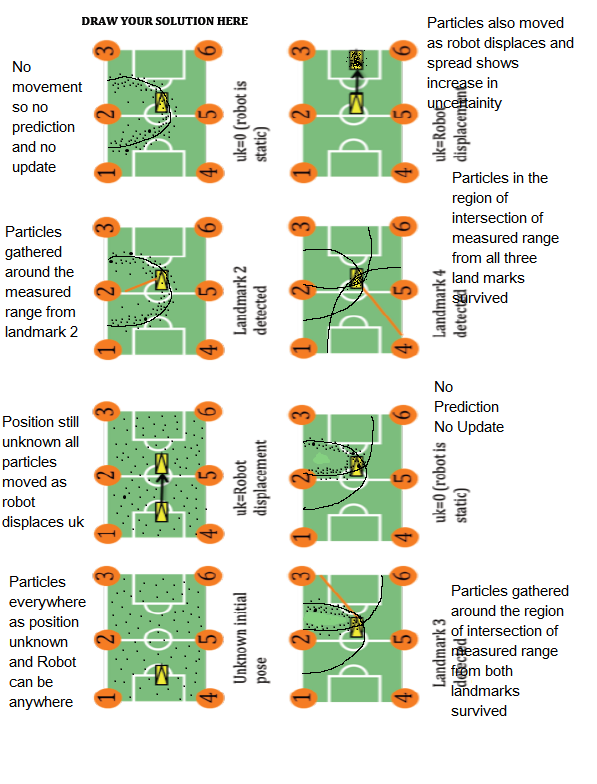
\includegraphics[width=0.7\textwidth]{solution2.png}
%
%\label{Solution22}
%\caption{Evolution of Particles}
%\end{figure}

\begin{thebibliography}{9}
\bibitem{1}
$http://www.fp.ucalgary.ca/mhallbey/what_is_texture.htm$
\bibitem{2}
Matlab Help
\bibitem{3}
$www.macs.hw.ac.uk/texturelab/files/publications/phds\_mscs/.../ch4.pdf$
\end{thebibliography}


\end{document}

 
